\documentclass[a4paper,12pt]{article}
\usepackage[utf8]{inputenc}
\usepackage[ngerman, english]{babel}
\usepackage{graphicx}
\usepackage{svg}
\usepackage{amsmath}
\usepackage{placeins}
\usepackage{geometry}
\usepackage{fancyhdr}
\usepackage[hidelinks]{hyperref}
\usepackage{longtable}
\usepackage[separate-uncertainty=true]{siunitx}
\usepackage{amsfonts}
\usepackage{enumitem}
\usepackage{multirow}
\usepackage{caption}
\usepackage{csquotes}
\usepackage[backend=biber]{biblatex}

\addbibresource{literature.bib} 


\captionsetup{labelfont=bf,tableposition=top}

\geometry{top=25mm,bottom=25mm,left=30mm,right=30mm}

% Font setup: Arial or Times New Roman
%\renewcommand{\rmdefault}{phv} % Arial
%\renewcommand{\rmdefault}{ptm} % Times New Roman

% Line spacing setup (1.5 line spacing)
\usepackage{setspace}
\onehalfspacing

% Make title block (cover page)
\begin{document}

% Title page
\begin{titlepage}
    \begin{center}
        \textbf{\Huge Experiment Protocol}\\[2cm]
        
        \textbf{\LARGE Module: Practical Biotechnology}\\
        \textbf{\large Practical part: Prof. Schillberg, BioVII}\\[2cm]
        
        \textbf{\LARGE Experiment: Heterologous Expression of mCherry in E. coli}\\[2cm]
        
        \textbf{\large Semester: Winter Semester 2024/25}\\[2cm]
        
        \textbf{\large Protocol Authors: }\\
        Kilian Mandon, Jonas Westphal, Florian Barkowski\\
        [2cm]
        
        \textbf{\large Submission Date: \today}
    \end{center}
\end{titlepage}

% Table of contents
\newpage
\tableofcontents
\newpage

% Section 1: Task Description
\section{Task Description}
The goal of the experiment was to assess the expression and purification of the protein mCherry in \emph{E. coli}. Concretely, the experiment aimed to elucidate whether the protein can be purified using affinity chromatography, detected by gel electrophoresis and Western Blot, quantified by the Enzyme-linked Immunosorbent Assay (ELISA) and measured at the transcriptome level using RNA extraction and Reverse Transcription Polymerase Chain Reaction (RT-PCR). These methods were applied to two constructs, mCherry-His and pelB-mCherry-His, to investigate differences in the expression and the expressed protein. The leader peptide pelB is supposed to guide the translated protein to the periplasm \cite{Sockolosky2013}. 

\section{Methods}
All experiments were carried out as described in the course notes. The primary data, the Python code for the quantitative analysis of the results, as well as the source code used to generate this document are available on GitHub\footnote{https://github.com/kilianmandon/mol-biotech-lab-course} up to four weeks after submission.

\section{Results}
\subsection{Expression and Isolation of mCherry}
Expression of mCherry in \emph{E. coli} was carried out both with and without a pelB leader peptide to test for differences in the expression behaviour. For the strain containing pelB-mCherry-His, the main culture reached an optical density (OD) of 0.622 2h47min after inoculation and expression was induced by addition of IPTG. For the strain containing mCherry-His, expression was induced 3h41min after inoculation at an OD of 0.584. For the strain with mCherry-His, the solution appeared violet both before and after induction, while the strain with mCherry-His was slightly yellow at both times.

The His-tagged proteins were thereafter purified using Immobilized Metal Affinity Chromatography (IMAC). After application of the lysed culture, the purification column used for the mCherry-His strain was violet, while the one used for pelB-mCherry-His remained colorless. Washing and flow-through fractions were colorless for both strains. The first elution fraction of the mCherry-His setup was colored violet, while all other elution fractions were colorless. 

The total protein concentration in the three elution fractions from affinity chromatography was determined with a Bradford Assay. For calibration, BSA protein solutions with known concentrations were used. After subtracting the absorbance of the used blank (Phosphate-buffered Saline, PBS), only the first elution of the pelB-mCherry-His construct and the first two elutions of the mCherry-His construct showed notable absorbance (Table \ref{tab:bradford1}). 

\begin{table}[h!]
    \centering
    \caption{\textbf{Bradford Assay: Absorbances of PelB and NonPelB Samples.} This table shows the blanked absorbances for PelB and NonPelB mCherry-His samples across the three elution fractions from affinity chromatography. The values represent the absorbance at 595 nm after blanking with the average absorbance of PBS. The three rows correspond to the dilutions 1:2, 1:5 and 1:10.}
    \begin{tabular}{ccc|ccc}
        \multicolumn{3}{c|}{\textbf{PelB (Absorbance)}} & \multicolumn{3}{c}{\textbf{NonPelB (Absorbance)}} \\
        \hline
        1st Elution & 2nd Elution & 3rd Elution & 1st Elution & 2nd Elution & 3rd Elution \\
        \hline
        0.1582 & 0.0001 & -0.0018 & 0.1755 & 0.0261 & 0.0013 \\
        0.0676 & -0.0081 & -0.0029 & 0.0569 & 0.0091 & -0.0036 \\
        0.0233 & -0.0130 & -0.0019 & 0.0231 & 0.0012 & 0.0014
    \end{tabular}
    \label{tab:bradford1}
\end{table}

The absorbance data for the calibration points followed a linear relation with a high coefficient of determination of $R^2 = 0.999$ (Figure \ref{fig:bradford1}). The linear model was determined as 
$$A = \SI{1.19}{\milli\liter\per\milli\gram} \cdot c + 0.0015$$

\begin{figure}[h!]
    \centering
    \includesvg[width=0.8\textwidth]{images/bradford_regression_plot.svg}  % Make sure to replace with your actual plot image file
    \caption{\textbf{Bradford Assay: Calibration Curve with Linear Regression. } Calibration was conducted using BSA protein solutions with known concentrations. Measured absorbances were plotted against the concentrations. The coefficient of determination was $R^2=0.999$.}
    \label{fig:bradford1}
\end{figure}

Protein concentrations in the elution fractions were estimated using the linear model and considering the dilution factors of the samples in the Bradford Assay. The second and third elution of the pelB construct as well as the third elution of the non-pelB construct showed no noticeable concentration of protein (Table \ref{tab:bradford2}). The first elution fractions of both constructs averaged out at about $\SI{240}{\micro\gram\per\milli\liter}$, while the concentration in the second elution from non-pelB was about $\SI{24}{\micro\gram\per\milli\liter}$. 



\begin{table}[h!]
    \centering
\caption{\textbf{Bradford Assay: Calculated Concentrations for PelB and NonPelB Samples.} This table presents the calculated concentrations for PelB and NonPelB mCherry-His. The concentrations were calculated based on the absorbance data using the linear regression model from calibration with BSA. The concentrations were further adjusted by multiplication with the dilution factor for each sample. The three rows correspond to the dilutions 1:2, 1:5 and 1:10.}
    \begin{tabular}{SSS|SSS}
        \multicolumn{3}{c|}{\textbf{PelB (µg/mL)}} & \multicolumn{3}{c}{\textbf{NonPelB (µg/mL)}} \\
        \hline
        {1st Elution} & {2nd Elution} & {3rd Elution} & {1st Elution} & {2nd Elution} & {3rd Elution} \\
        \hline
        263.47 & -2.32 & -5.43 & 292.46 & 41.46 & -0.31 \\
        278.01 & -40.05 & -18.41 & 232.85 & 32.01 & -21.14 \\
        183.34 & -121.70 & -28.42 & 182.08 & -2.37 & -0.27 
    \end{tabular}
    \label{tab:bradford2}
\end{table}

For each of these three elutions, the measurements had high variance within the different dilutions in the Bradford Assay, driven mostly by the lowest dilution of 1:20. Protein concentration in the first elution of the pelB construct was determined as $\SI{241.61\pm 41.63}{\micro\gram\per\milli\liter}$, in the first elution of the non-pelB construct as $\SI{235.80\pm 45.11}{\micro\gram\per\liter}$ and in the second elution of the non-pelB construct as $\SI{23.70 \pm 18.83}{\micro\gram\per\liter}$ (Table \ref{tab:bradford3}).

\begin{table}[h!]
    \centering
    \caption{\textbf{Bradford Assay: Average and Standard Deviation of Adjusted Concentrations for PelB and NonPelB Samples.} This table summarizes the average and standard deviation of the adjusted concentrations (after multiplication with concentration factors) for PelB and NonPelB mCherry-His, grouped by the three elution fractions.}
    \begin{tabular}{lccc}
        & \textbf{1st Elution} & \textbf{2nd Elution} & \textbf{3rd Elution}\\
        \hline
        \textbf{PelB (µg/mL)} & 241.61 $\pm$ 41.63 & -54.69 $\pm$ 49.82 & -17.42 $\pm$ 9.41 \\
        \textbf{NonPelB (µg/mL)} & 235.80 $\pm$ 45.11 & 23.70 $\pm$ 18.83 & -7.24 $\pm$ 9.83  \\
        \hline
    \end{tabular}
    \label{tab:bradford3}
\end{table}

\subsection{SDS PAGE and Western Blot}
To determine the composition of the previously measured protein and to check for the presence of the constructs pelB-mCherry-His and mCherry-His, an analysis using SDS-PAGE and Western Blotting was conducted. Our group conducted the experiments for the pelB construct, while the data for the non-pelB construct shown in this protocol was measured by Group 6.

In the SDS analysis, the positive control mCherry-His created a large band at around 34~kDa (in the pelB experiment) and 30~kDa (in the non-pelB experiment) respectively, as well as two smaller bands at about 32 kDa and 24 kDa (in the pelB experiment, slightly lower values and less prominent bands were observed in the non-pelB experiment). All three bands were visible in the Western Blot in both experiments (Figures \ref{fig:sds_pelB} and \ref{fig:sds_non_pelB}). 

\begin{figure}[!htbp]
    \centering
    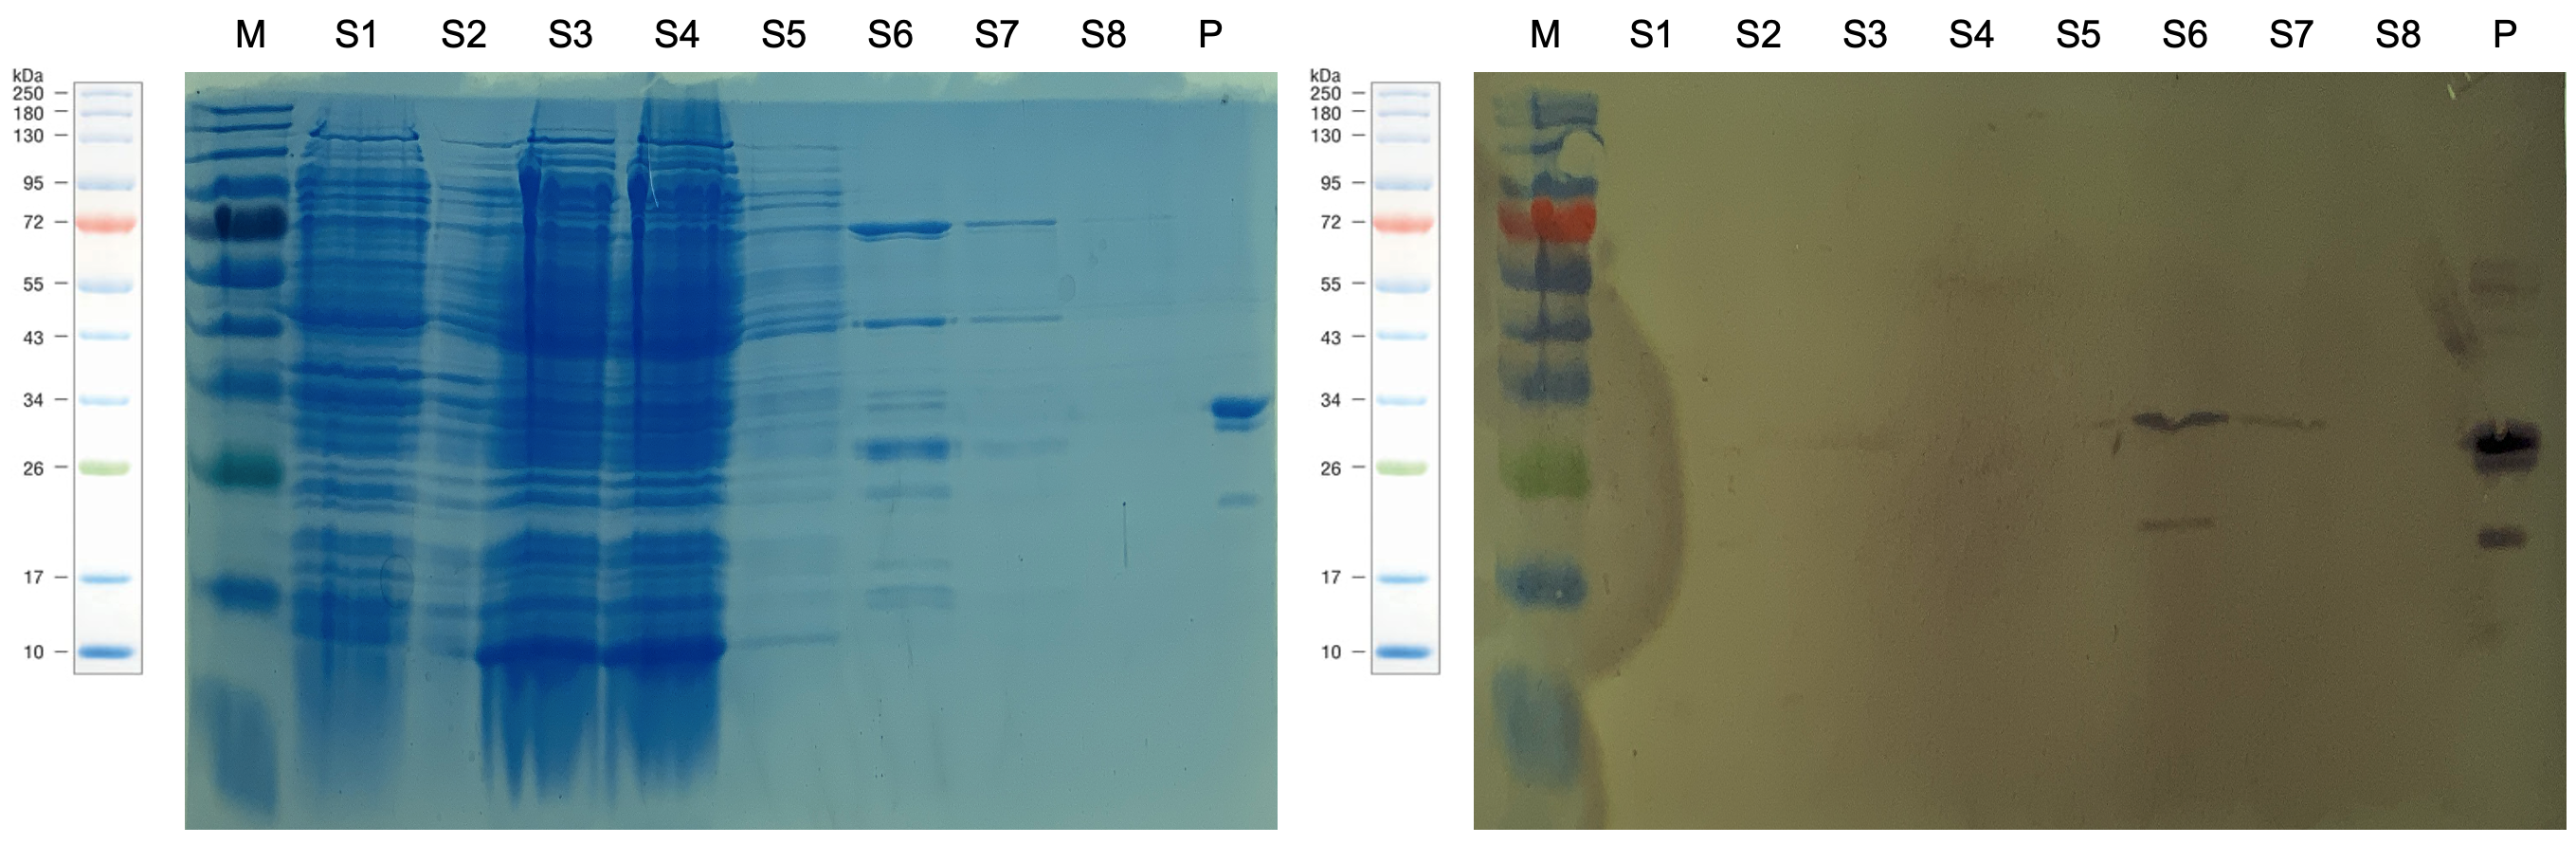
\includegraphics[width=\textwidth]{images/sds_western_blot.png}
    \caption{\textbf{SDS-PAGE and Western Blot of PelB-mCherry-His during different steps of purification.} Track M contains the marker \emph{Color Prestained Protein Standard, Broad Range (10-250 kDa)} by NEB. Track P contains mCherry-His as positive control. The tracks S1 to S8 contain, in this order, a sample from the main culture before induction (1, no lysis), after induction (2, no lysis), after induction and sonification (3), as well as samples from the flow-through fraction (4), the washing fraction  (5) and three elution fractions (6-8) from IMAC. }
    \label{fig:sds_pelB}
\end{figure}

The tracks S1 to S4 contained, in this order, samples from the cell culture before and after induction, from the supernatant after lysis, and from the flow-through fraction from affinity chromatography. In both experiments, all four showed a largely continuous spectrum of proteins with larger bands in the tracks S3 and S4 (after lysis). For the pelB construct, the tracks S1 to S4 showed little to know signals in the Western Blot. For the non-pelB construct, all four tracks showed two strong bands at similar weights as the positive control (~32 kDa and ~24 kDa). The bands were less prominent in the flow-through fraction.

\begin{figure}[!htbp]
    \centering
    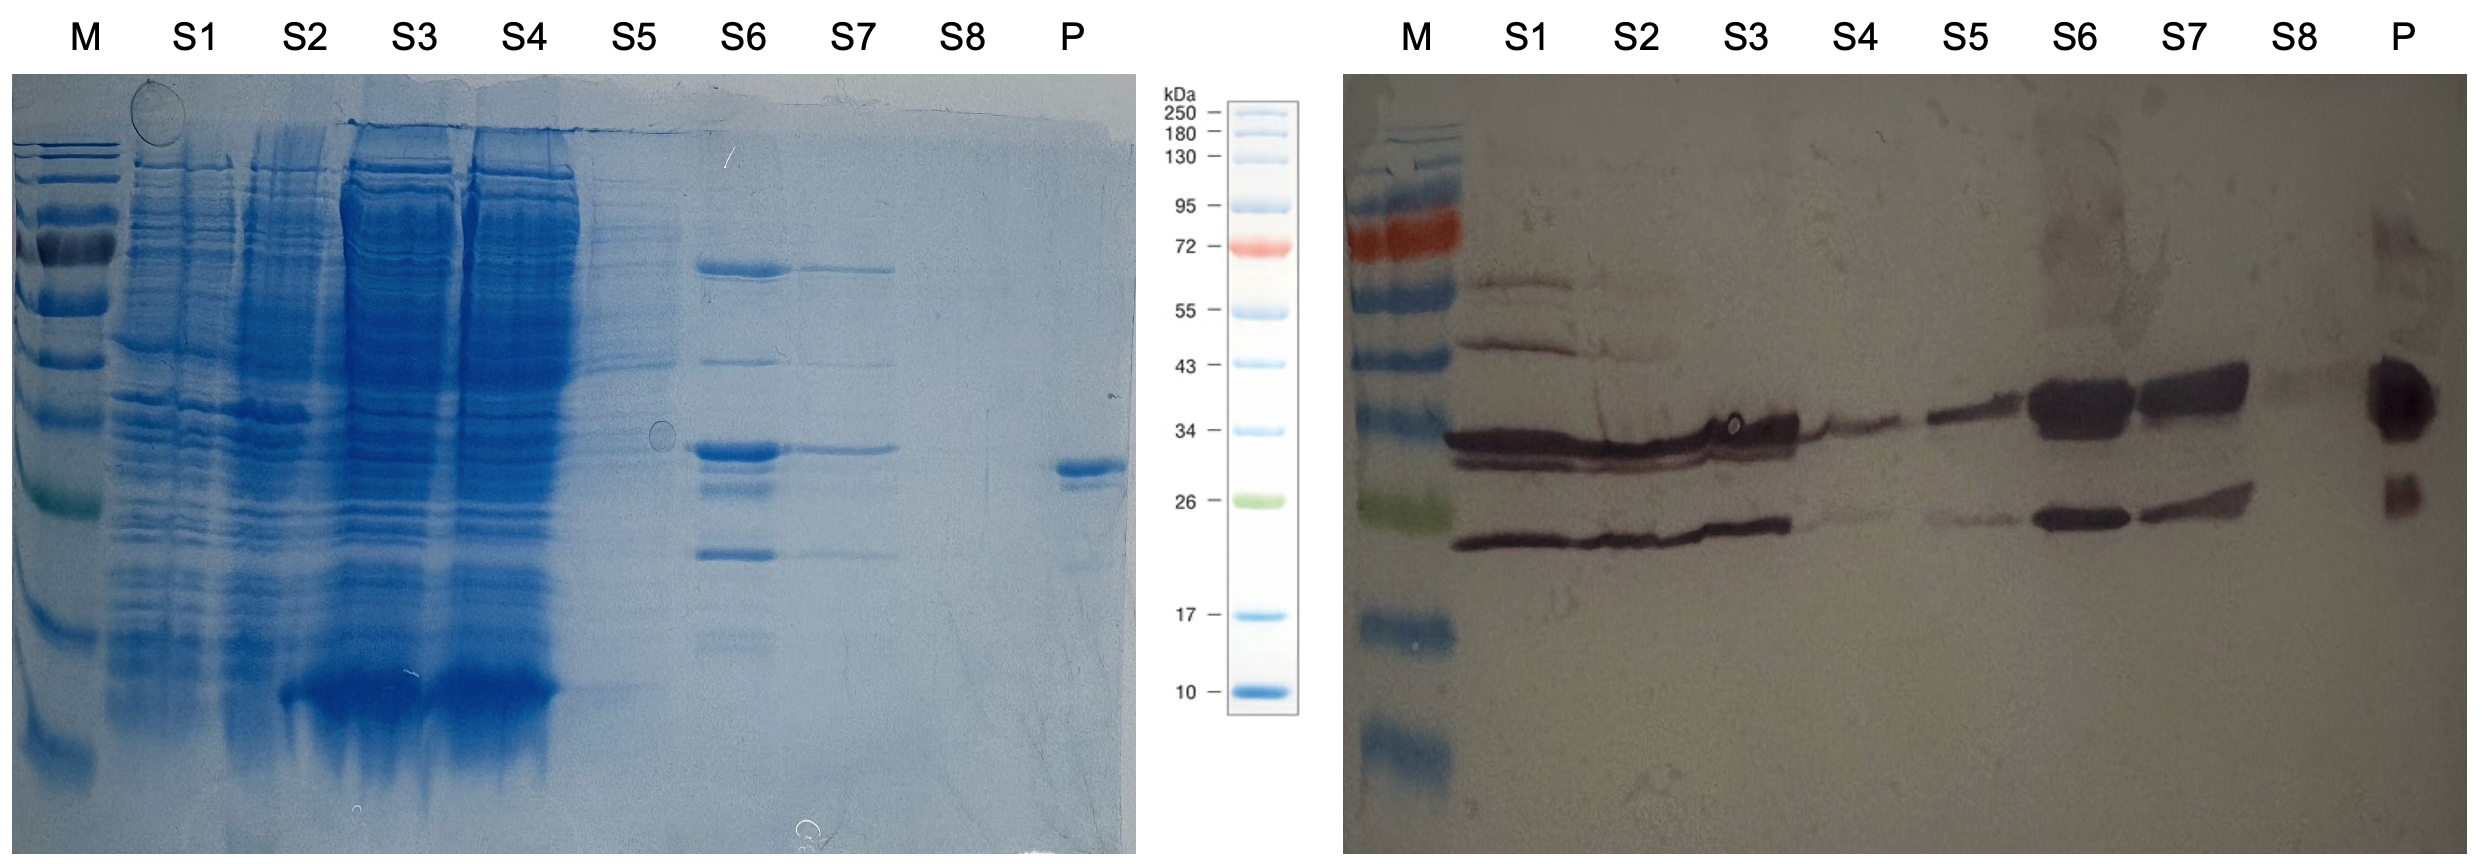
\includegraphics[width=\textwidth]{images/group6_sds_western.png}
    \caption{\textbf{SDS-PAGE and Western Blot of mCherry-His during different steps of purification.} Track M contains the marker \emph{Color Prestained Protein Standard, Broad Range (10-250 kDa)} by NEB. Track P contains mCherry-His as positive control. The tracks S1 to S8 contain, in this order, a sample from the main culture before induction (1, no lysis), after induction (2, no lysis), after induction and sonification (3), as well as samples from the flow-through fraction (4), the washing fraction  (5) and three elution fractions (6-8) from IMAC. }
    \label{fig:sds_non_pelB}
\end{figure}

The tracks S5 to S8 contained samples from the washing step during affinity chromatography, as well as from the three elution fractions. In both experiments, the washing fraction showed a large number of discrete, faint bands in the SDS gel. For the pelB construct, the first elution fraction showed a number of discrete, faint bands, as well as three particularly strong bands (at weights of 72 kDa, 50 kDa and 30 kDa). The second elution fraction had similar bands to the first one, but fainter. The third elution fraction showed no bands in the SDS gels. For the non-pelB construct, the tracks appeared similar to those of pelB, showing pronounced bands at weights of 72~kDa, 34~kDa and 20~kDa. The band at 34~kDa was particularly prominent in the SDS gel. The second elution showed the same pattern with fainter bands, and the third elution showed no visible bands.

In the Western Blot, the pelB construct showed prominent bands at 34~kDa  and a faint band at 24~kDa in the first elution fraction, as well as a faint band at 34~kDa in the second elution fraction. For the non-pelB construct, the washing fraction showed bands at 34~kDa and a faint band at 24~kDa, while the first two elutions showed strong bands at both corresponding weights. The third elution fraction showed a faint band at a weight of 34~kDa. Both SDS gels and the corresponding Western Blots showed horizontal curvature.





\subsection{ELISA Assay}
For a quantitative analysis of the specific concentration of mCherry-His in the elution fractions, an ELISA assay was performed. After application of the primary and secondary antibody, the samples were incubated with the substrate nitrophenyl phosphate for 15 minutes before absorbance measurement. For the non-pelB construct, the absorbance of the samples from the first two elution fractions exceeded the device's measurement range in all three dilutions. The absorbances of the third elution were measured as about 3.7, 2.5 and 1.1 for the three dilutions 1:5, 1:10 and 1:20 respectively. For the pelB construct, all three elutions were measurable by the photometer. The measured absorbances for the first elutions are similar to those of the third elution from the non-pelB construct. The second and third elutions had little to no absorbance (Table \ref{tab:elisa1}). Note that the non-pelB measurements do not correspond to the SDS-PAGE and Western Blot results presented in the last section, as those were conducted by a different group.

\begin{table}[h!]
    \centering
    \caption{\textbf{ELISA Assay: Absorbances of PelB and NonPelB Samples.} This table shows the blanked absorbances for PelB and NonPelB mCherry-His samples across the three elution fractions from affinity chromatography. Before measurement, the samples were incubated with the primary and secondary antibody, as well as the substrate nitrophenyl phosphate. The values represent the absorbance at 405~nm after blanking with the average absorbance of the coating buffer. The three rows correspond to the dilutions 1:5, 1:10 and 1:20. Values exceeding the device's measurement range are denoted as High.}
    \begin{tabular}{SSS|SSS}
        \multicolumn{3}{c|}{\textbf{PelB (Absorbance)}} & \multicolumn{3}{c}{\textbf{NonPelB (Absorbance)}} \\
        \hline
        {1st Elution} & {2nd Elution} & {3rd Elution} & {1st Elution} & {2nd Elution} & {3rd Elution} \\
        \hline
        3.151 & 0.445 & -0.067 & {High} & {High} & 3.652 \\
        2.162 & 0.103 & -0.067 & {High} & {High} & 2.460 \\
        1.214 & -0.016 & 0.036 & {High} & {High} & 1.058 
    \end{tabular}
    \label{tab:elisa1}
\end{table}

\newpage
As for the Bradford Assay, a linear model for the relationship between absorbance and concentration was created based on samples with known concentrations of mCherry-His. The calibration data generally followed a linear trend with a coefficient of determination of $R^2 = 0.94$ (Figure \ref{fig:elisa1}). The linear model was determined as 
$$A = \SI{3.76}{\milli\liter\per\micro\gram} \cdot c + 0.057$$

\begin{figure}[h!]
    \centering
    \includesvg[width=0.8\textwidth]{images/elisa_regression_plot.svg}  % Make sure to replace with your actual plot image file
    \caption{\textbf{ELISA Assay: Calibration Curve with Linear Regression. }  Calibration was conducted using mCherry-His protein solutions with known concentrations. Measured absorbances were plotted against the concentrations after subtracting the blank value. The coefficient of determination was $R^2=0.94$. Absorbances for the highest two concentration exceeded the device's measurement range and are not included in the chart.}
    \label{fig:elisa1}
\end{figure}

Applying the linear model to the measured absorbances for the pelB and non-pelB construct and considering the dilution factors, concentrations of pelB-mCherry-His and mCherry-His were estimated for the three elution fractions. Corresonding to the absorbances, concentration in the first two elution fractions from the non-pelB construct exceeded the measurement range of the photometer, while the second and third elution of the pelB construct showed no significant concentration (Table \ref{tab:elisa2}). 

\begin{table}[h!]
    \centering
\caption{\textbf{ELISA Assay: Calculated Concentrations for PelB and NonPelB Samples.} This table presents the calculated concentrations for PelB and NonPelB mCherry-His. The concentrations were calculated based on the absorbance data using the linear regression model from calibration with mCherry-His. The concentrations were further adjusted by multiplication with the dilution factor for each sample. The three rows correspond to the dilutions 1:5, 1:10 and 1:20. Values exceeding the device's measurement range are denoted as High.}
    \begin{tabular}{SSS|SSS}
        \multicolumn{3}{c|}{\textbf{PelB (ng/mL)}} & \multicolumn{3}{c}{\textbf{NonPelB (ng/mL)}} \\
        \hline
        {1st Elution} & {2nd Elution} & {3rd Elution} & {1st Elution} & {2nd Elution} & {3rd Elution} \\
        \hline
        4.11 & 0.52 & -0.16 & {High} & {High} & 4.78 \\
        5.59 & 0.12 & -0.33 & {High} & {High} & 6.38 \\
        6.14 & -0.39 & -0.11 & {High} & {High} & 5.32 \\
    \end{tabular}
    \label{tab:elisa2}
\end{table}

The first elution of pelB and the third elution of non-pelB were determined as similar concentrations. Concretely, the concentration in the first elution of the pelB construct averaged out as $\SI{5.28\pm 0.86}{\micro\gram\per\milli\liter}$, while the third elution of the non-pelB construct was measured as $\SI{5.49 \pm 0.67}{\micro\gram\per\milli\liter}$ (Table \ref{tab:elisa3}).

\begin{table}[h!]
    \centering
    \caption{\textbf{ELISA Assay: Average and Standard Deviation of Adjusted Concentrations for PelB and NonPelB Samples.} This table summarizes the average and standard deviation of the adjusted concentrations (after multiplication with concentration factors) for PelB and NonPelB mCherry-His, grouped by the three elution fractions. Values exceeding the device's measurement range are denoted as High.}
    \begin{tabular}{lccc}
        & \textbf{1st Elution} & \textbf{2nd Elution} & \textbf{3rd Elution}\\
        \hline
        \textbf{PelB (µg/mL)} & 5.28 $\pm$ 0.86 & 0.08 $\pm$ 0.37 & -0.20 $\pm$ 0.09 \\
        \textbf{NonPelB (µg/mL)} & High  & High & 5.49 $\pm$ 0.67  \\
        \hline
    \end{tabular}
    \label{tab:elisa3}
\end{table}

\subsection{RNA Extraction}
In addition to the analysis of expression on protein-level, Total RNA Extraction and RT-PCR were carried out for the analysis of the corresponding transcriptome. Both experiments were conducted with the \emph{E. coli} strain containing pET22b-mCherry-His. 

After the Total RNA Extraction assay (performed in duplicate), RNA concentrations in the two samples were determined using a NanoDrop spectrophotometer as $\SI{401.5}{\nano\gram\per\micro\liter}$ and $\SI{325.8}{\nano\gram\per\micro\liter}$. Both samples had an A260/A280 absorbance ratio of 2.06 (Table \ref{tab:rna1}). 

\begin{table}[h!]
\centering
\caption{\textbf{Concentration and Absorbance Measurement After Total RNA Extraction} from an \emph{E. coli} strain containg pET22b-mCherry-His. The measurement was carried out using a NanoDrop spectrophotometer. }
\begin{tabular}{lcccc}
    & \textbf{Concentration (ng/µL)} & \textbf{A260} & \textbf{A280} & \textbf{A260/A280} \\
    \hline
    Sample 1 & 401.5 & 10.04 & 4.87 & 2.06 \\
    Sample 2 & 325.8 & 8.15 & 3.95 & 2.06 
\end{tabular}
\label{tab:rna1}
\end{table}

Following Total RNA Extraction, the samples were analyzed using agarose gel electrophoresis. Both samples, as well as the positive control, showed strong bands at 2900~bp and 1500~bp, as well as a faint band with less than 200~bp. The two bands at 2900~bp and 1500~bp are particularly pronounced for the positive control, where they are both followed by a slightly diffuse region below them (Figure \ref{fig:rna1}).

\begin{figure}[h!]
    \centering
    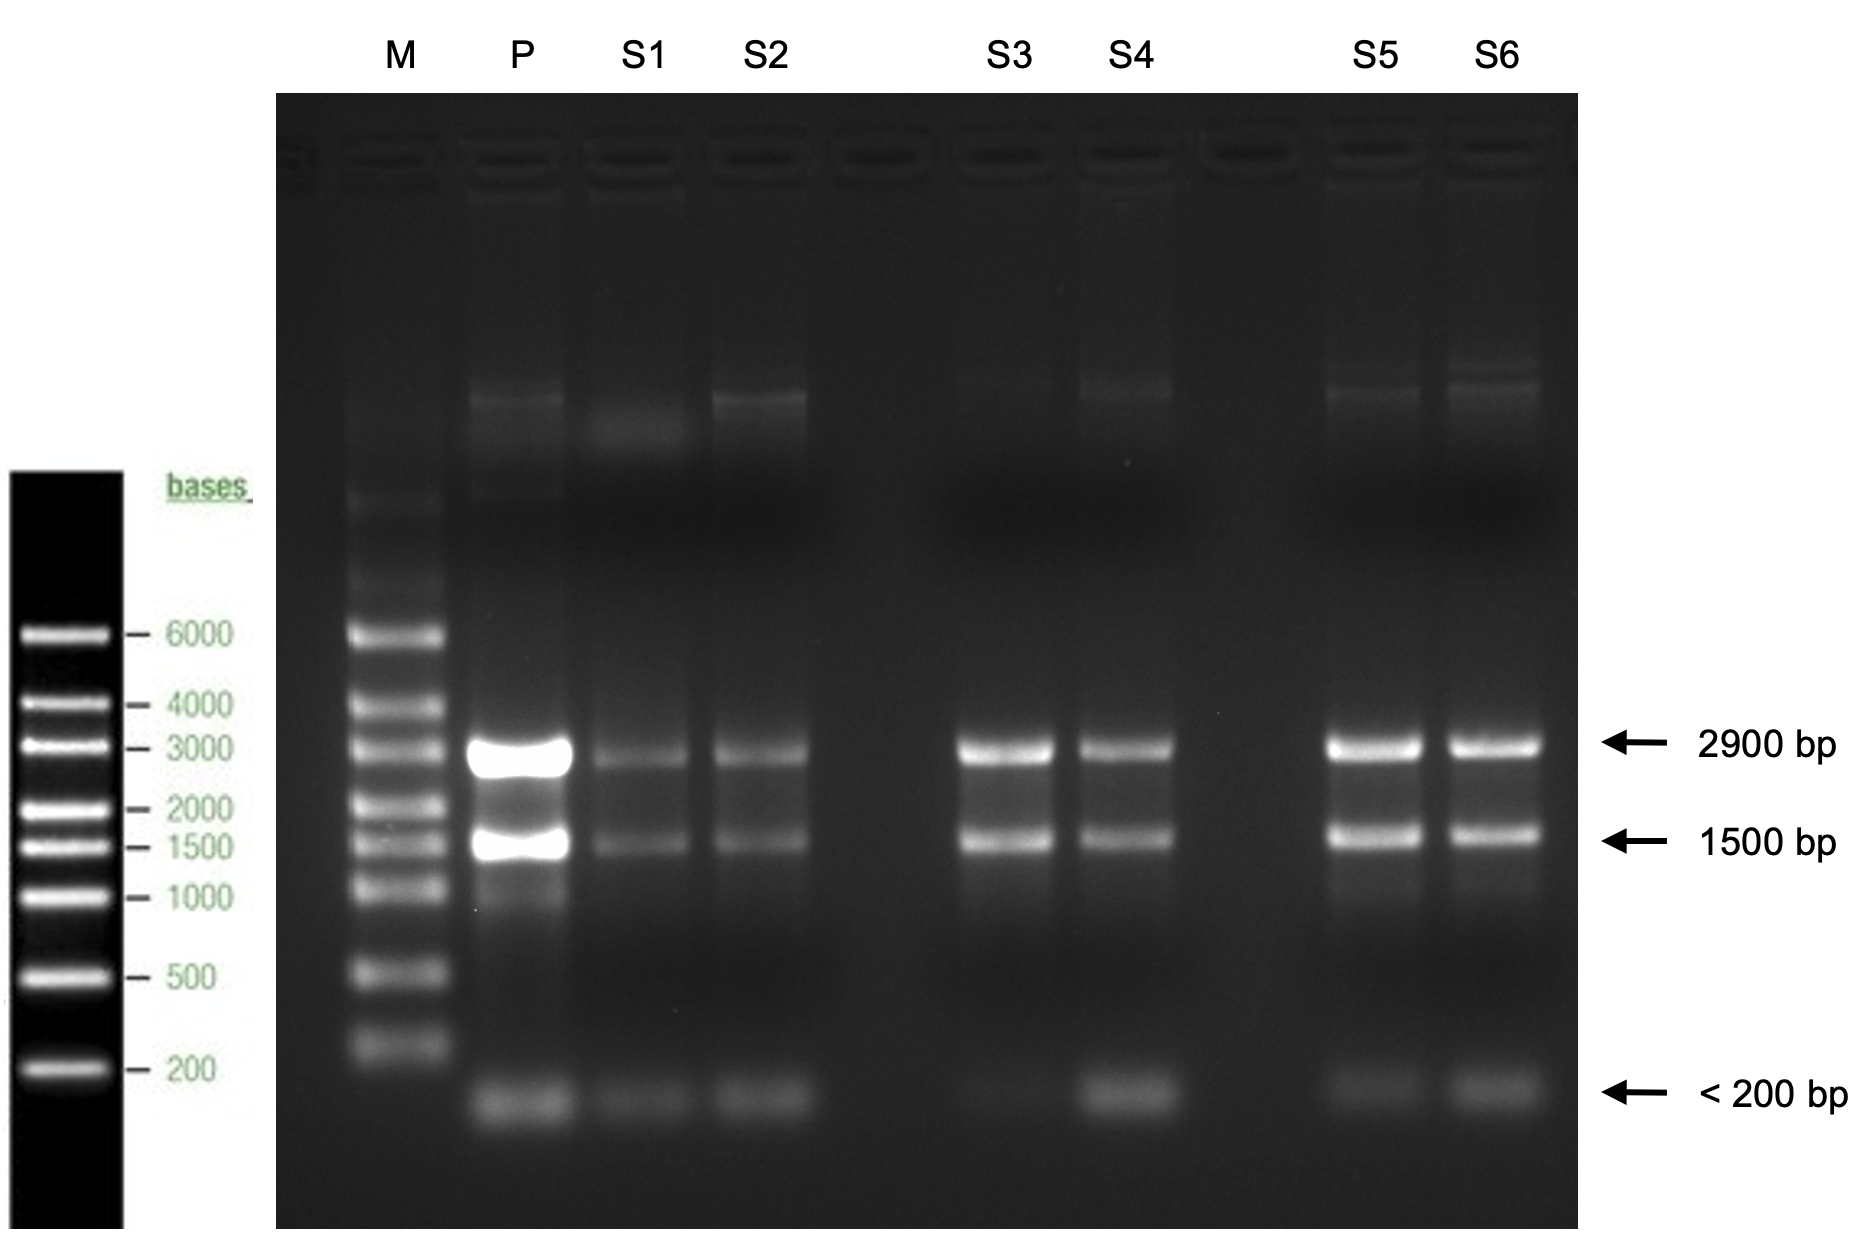
\includegraphics[width=\textwidth]{images/rna_pre_pcr.png}
    \caption{\textbf{Agarose Gel Electrophoresis Following Total RNA Extraction} from an \emph{E. coli} strain containing pET22b-mCherry-His. Track M contains the marker \emph{RiboRuler High Range RNA Marker} by Thermo Fisher Scientific. Track P contains previously extracted total RNA from \emph{E. coli} as positive control. The tracks S1 to S4 contain samples from extraction by different groups. The tracks S5 and S6 contain the elution fraction from the purification, which was performed in duplicate. }
    \label{fig:rna1}
\end{figure}

The samples from Total RNA Extraction underwent DNase treatment and reverse transcription. Samples from before and after DNase treatment, after reverse transcription, as well as water and pET22b-mCherry-His plasmid DNA as negative and positive control, were used in a PCR with primers for mCherry. In the following agarose gel electrophoresis, the samples taken before DNase treatment and after reverse transcription, as well as the positive control, showed bands at 740~bp. The sample taken after DNase treatment showed a faint band at the same migration distance (Figure \ref{fig:rna2}).

\begin{figure}[h!]
    \centering
    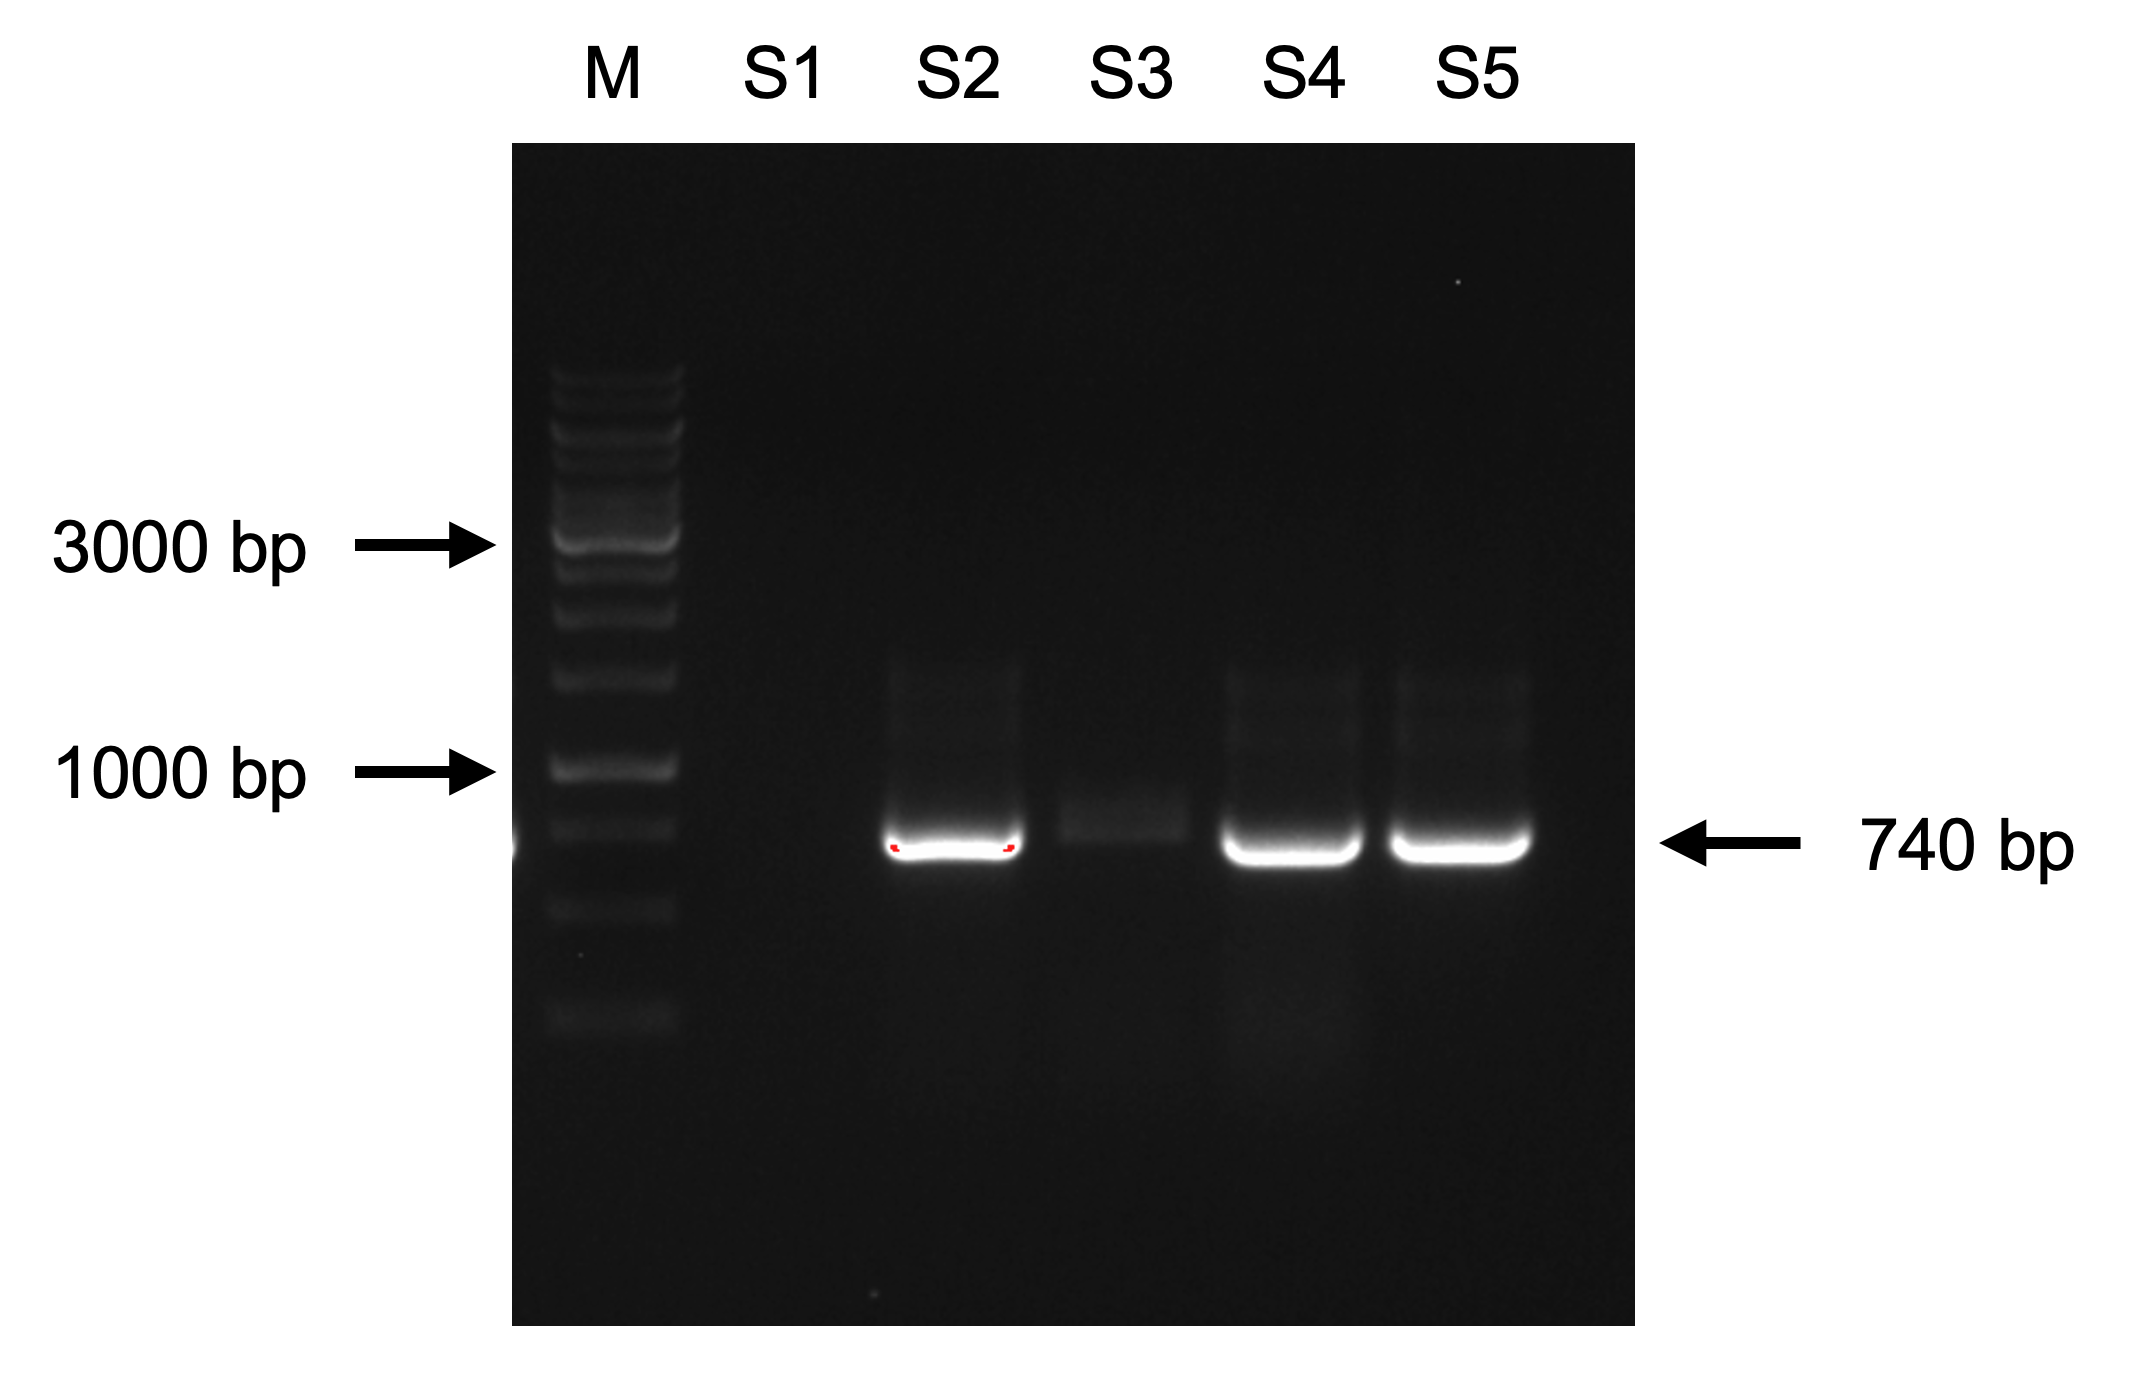
\includegraphics[width=\textwidth]{images/rna_post_pcr.png}
    \caption{\textbf{Agarose Gel Electrophoresis Following RT-PCR.} The samples used as templates for PCR are from different stages of Total RNA Extraction from an \emph{E. coli} strain containing pET22b-mCherry-His. Track M contains the marker \emph{GeneRuler 1kb DNA Ladder} by Thermo Fisher Scientific. Templates used for the PCR in the tracks S1 to S5 are, in this order, H\textsubscript{2}O, cDNA (after RT), total RNA after DNase treatment, total RNA before DNase treatment, and pET22b-mCherry-His plasmid DNA (positive control). The tracks S2, S4 and S5 show a band at 740~bp. Track S3 shows a faint band at the same migration distance.}
    \label{fig:rna2}
\end{figure}
% Section 4: Discussion
\FloatBarrier
\section{Discussion}
\subsection{Expression and Isolation of mCherry}
Both mCherry-His and pelB-mCherry-His were expressed in \emph{E. coli} BL21 (DE3) to investigate heterologous expression and the influence of the pelB leader sequence. The strain expressing mCherry-His already appeared violet before induction, which indicates expression of mCherry-His. In the expression system, mCherry-His is under control of the T7-Promoter, which can only be transcribed by the T7-Polymerase. In \emph{E. coli} BL21 (DE3), the T7-Polymerase is under the control of the lacUV5 promoter, which is known to be leaky \cite{du2021regulating}. This is a probable cause for the violet color of the cell culture before induction with IPTG. 

The strain with pelB-mCherry-His remained uncolored both before and after induction. However, the Bradford Assay on the elution fractions of IMAC showed a similar protein concentration in the first elution fractions for both the pelB and  the nonPelB construct. Presence of protein in the elution fraction indicates that the strain with pelB-mCherry-His expressed proteins that remained attached to the column during washing. These could be both specific interactions of proteins with a His-Tag, which is only present in the pelB-mCherry-His construct in this strain, as well as unspecific interactions of other proteins containing suitable amino acids (in particular histidine).

\subsection{SDS PAGE and Western Blot}
To further investigate on the nature of the proteins purified by IMAC, SDS-PAGE and a Western Blot were conducted to analyze the weight of the protein, as well as their specific interaction with anti-His-antibodies. For both constructs, samples from the culture before and after induction with IPTG, as well as samples after cell lysis and from the flow-through fraction from affinity chromatography, showed a broad spectrum of bands in the SDS gel. The missing specificity of the bands is expected, given that no purification was conducted. Presence of bands in the tracks of the non-lysed samples indicates that soluble protein was contained in the samples at the point of time when the PAGE was conducted. These could both be secreted proteins, as well as products from a partial lysis by the SDS sample buffer. However, in both experiments, the gel showed stronger bands for the samples after cell lysis, indicating that SDS sample buffer isn't sufficient for a complete lysis and that the sonification effectively contributed to freeing intracellular proteins. 

The washing fraction showed little amount of protein, meaning that aside of the strongly interacting proteins in the elution fractions, there were few proteins with an intermediate amount of affinity to the IMAC column. The three elution fractions appeared similar in the SDS-PAGE for both constructs, suggesting that the presence of the bands not coinciding with the positive control is systematic. In particular the band at 72~kDa, having a molecular weight higher than the positive control, could not have arisen from cleavage of mCherry-His and suggests the presence of a specific protein in the strain with high affinity to the IMAC column.

The two experiments strongly differed in the Western Blot. For the pelB-mCherry-His construct, only two faint bands were present in the first elution fraction and at weights corresponding to that of the positive control. While this shows that pelB-mCherry-His was in fact expressed, it also suggests that this was only the case in relatively low amounts. The high protein concentration in the elution fraction as measured in Bradford likely arose from proteins that had relatively strong unspecific interactions with the IMAC column, whilst not interacting with the anti-His-antibodies used in the Western Blot. 

For the experiment using mCherry-His, the Western Blot showed strong bands for proteins corresponding to the two bands from the positive control throughout all steps of the purification, with less pronounced bands for the flow-through and washing fractions. This shows that mCherry-His was successfully expressed and purified. The lower presence in the flow-through and washing fractions is likely due to the strong interaction of mCherry-His with the IMAC column, holding it back in the column. The presence of the two separate bands in the test samples as well as the positive control might come from proteolytic cleavage of mCherry-His, creating a lighter version of the protein that still contains the His-Tag and can thus be bound by the anti-His-antibody. For mCherry-His, the first track also showed two bands at higher molecular weight, which suggests the expression of proteins with a higher molecular weight than mCherry-His that were also bound by the anti-His-antibodies. However, the bands weren't present in any other sample and it is unclear why such proteins should be lost in the following steps. Thus, the existence of such proteins shouldn't be taken as fact until further experiments show supporting results.

The weight of the most pronounced bands from the positive control mCherry-His were at 34~kDa and 30~kDa for the two experiments. The expected molecular weight of mCherry-His without a pelB leader is 28~kDa, which is below the observed values. The corresponding weight of the most pronounced bands in the elution fractions from the two experiments was 34~kDa for both the pelB and the non-pelB construct. The deviation of weight of the positive control in the two experiments exceeded the difference between the theoretical molecular mass of the pelB construct (30.2~kDa) and the non-pelB construct (28.0~kDa). The fact that all measured values exceeded both theoretical weights could be due to sagging of the gel, as observed by the horizontal curvature, and could be mitigated by more careful treatment of the gels. A significant difference of the weights for the pelB and the non-pelB construct could not be observed. This could indicate proper processing of the pelB construct, which is supposed to undergo cleavage of the leader peptide after successful translocation to the periplasm \cite{Sockolosky2013}. However, given the large deviation of the observed molecular weights from their theoretical ones, this is no sure result and needs further evidence. A repetition of the experiment with more careful handling and additional intermediate marker tracks could help, but the difference in weight of 2~kDa might still be too narrow for resolution using gel electrophoresis.


\subsection{ELISA Assay}
For further analysis of the protein composition in the elution fractions from affinity chromatography, an ELISA assay using primary anti-His-antibodies was conducted for both the pelB and the non-pelB construct. The measurement for the non-pelB construct exceeded the measurent range of the photometer, showing a high presence of mCherry-His in the elution. The calculated concentration of pelB-mCherry-His in the first elution fraction was about the same as for the third elution fraction from the non-pelB construct, even though this third elution fraction contained no significant amount of protein according to the Bradford Assay. This supports the claim that the strain containing pelB-mCherry-His expressed very little of the protein, and that the high amount of protein in the first elution fraction of the pelB construct was made up by proteins with non-specific interactions with the IMAC column. 

Given the problems with the measurement range, the ELISA Assay failed to provide quantitative results for the non-pelB construct and could only further establish the qualitative result from the Western Blot that the samples contained significant amounts of antigen for the anti-His-antibodies. For a quantitative analysis, the assay should be repeated using increased dilution or a shorter incubation with the substrate PNPP.

\subsection{RNA Extraction}
For analysis of the transcriptome, Total RNA Extraction and RT-PCR were conducted. Both samples, as well as the positive control, showed strong bands at 2900~bp and 1500~bp, as well as a fainter band corresponding to a length less than 200~bp. These values coincide with the reported lengths of the 23S rRNA (2904~bp) and the 16S rRNA (1542~bp), while the low-molecular band might come from the 5S rRNA (120~bp) from \emph{E. coli} \cite{Kaczanowska2007}. rRNAs are the most abundant RNAs in the cell, often making up 80\% to 90\% of the cell's total RNA \cite{Munafo2016}. Thus, it is highly likely that the observed bands in fact arose from those rRNAs. The slight smearing below the bands at 2900~bp and 1500~bp in the positive control might indicate partial degradation of the RNA. The observed absorbance ratio of $\text{A260}/\text{A280}=2.06$ is close to the value of 2.0, which is typically associated with high quality RNA without protein contamination \cite{poovakka2018quality}. 

In the following RT-PCR, the samples containing cDNA, total RNA without DNase treatment and the positive control showed strong bands at 740~bp. This matches the expected size of the construct of 734~bp \cite{Schillberg2025}, showing that the primers could specifically bind and amplify both the cDNA and genomic DNA encoding the protein. It also shows that the mRNA for mCherry-His was in fact present in the total RNA, corresponding to the proof of expression on the proteome-level using ELISA and Western Blot. The track containing total RNA after DNase treatment shows a very faint band. This suggests that while the DNase could effectively degrade most of the genomic DNA, there were still DNA molecules present that could be amplified by the PCR. Given the exponential nature of PCR amplification, this small amount is expected to largely increase with a higher number of PCR cycles, which could be investigated when repeating the experiment.

\section{Conclusion}
The experiments could successfully assess the expression of mCherry-His in \emph{E. coli}. The SDS-PAGE and Western Blot could effectively demonstrate the purity of mCherry-His after IMAC. Although the ELISA was unable to quantify the expression due to an improper measuring range, it further established the presence of mCherry-His in the purified sample with high concentration. In addition to the proteomic analysis, Total RNA Extraction and RT-PCR were able to prove transcription of the construct. 

For the pelB-construct, the SDS-PAGE of the elution fractions showed protein, indicating the presence of proteins with high affinity to the Ni-NTA column. However, immunogenic analysis using ELISA and Western Blot targeting the His-tag only lead to weak signals. Together with the absence of color in the samples, this suggests that the protein was either not expressed in high amounts, rapidly degraded by the cell, or improperly folded in a way that hindered both the protein's fluorescence as well as binding of its His-tag to anti-His-antibodies. Previous experiments by \cite{linton2012translocation} investigated pelB fusion proteins with another fluorescent protein, eGFP, and found that the pelB-eGFP proteins lead to inactive, non-fluorescent eGFP that was mostly trapped in the inner membrane. It is possible that the pelB-mCherry construct used in this experiment did likewise. The authors showed that a different signal peptide, TorA, effectively translocated eGFP to the periplasm. For further experiments, it might be interesting to assess whether this construct would lead to different outcomes for the mCherry constructs.


\section{References}
\printbibliography[heading=none]


% Section 6: Declaration of Independence
\newpage
\section*{Declaration of Independence}
I hereby declare that I have completed the experiment and written this protocol independently. I have not received unauthorized assistance and have properly cited all sources. Furthermore, I have used AI-based programs for grammar checking and formatting purposes only.

Date: \today \\
Signature: \underline{\hspace{5cm}}

\end{document}